\section{Design and solution}
\label{sec:middleware_architecture}
Before assessing the elicited requirements and incorporating the decisions as part of the solution, a thorough description of the design is to be conducted and presented in relevance to the stated quality attributes. Software architecture consolidates a collection of different architectural patterns that can be utilised as blueprints to solve a specific problem and identify proper structure within the many levels of a complex system. The selection of what patterns as well as tactics to be used to accommodate the mitigation of a specific problem depends on the system to be developed and deployed. For the project, the domain was to design a complex system in relation to Industry 4.0 production, through the incorporation of different architectures and technologies. The consideration of software architecture meant that architectural challenges in the system had to be considered, while designing how production components would interact with each other to achieve some common tasks. As intended, the design initialized were to accommodate a selection of key quality attributes composed of interoperability, availability, deployability as well as performance, while the software constituting the production software would run 24/7 and be continuously deployable. Before analyzing the specified tactics and patterns utilised, the overall design and architecture were to accommodate the workflow proposed in figure \ref{fig:flow-diagram}.

\begin{figure}[!htb]
    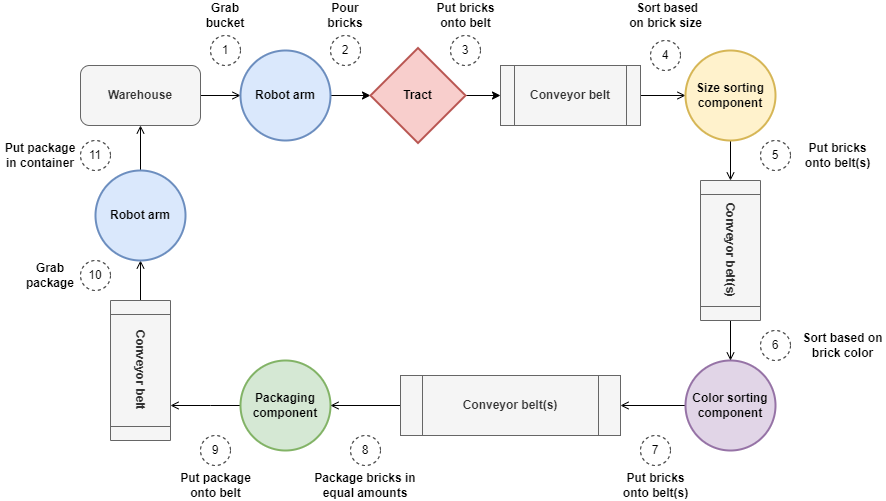
\includegraphics[width=250pt]{images/flow-diagram.png}
    \caption{Flow diagram of production system}
    \label{fig:flow-diagram}
\end{figure}

\subsubsection{System hierarchy}
Throughout the development of the production software, several systems of both primary and secondary proportion had to be considered to comply with the nature of managing the design of a complex Cyber-Physical system. The hierarchy would consolidate of four primary systems, 1) Production Management System (PMS), 2) Supply Chain Management System (SCMS), 3) Robotics, and 4) Internet of Things (IoT) appliances; however, each primary system would be responsible for one or more secondary systems, as shown in figure \ref{fig:hierarchy}. The adjustment of secondary systems that had to meet the needs of a parent system introduced the challenge of various independent but loosely coupled systems, that had to be interconnected in a flexible manner. This would promote the mindset of utilising a generalised microservice architecture for the production software.  
\newpage
\begin{figure}[!htb]
    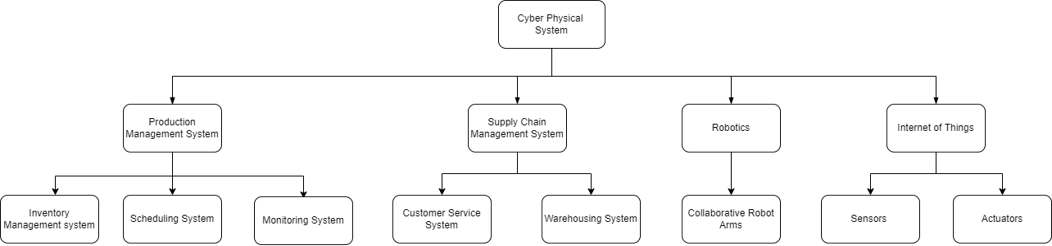
\includegraphics[width=250pt]{images/hierarchy.png}
    \caption{Initial hierarchy diagram of production system}
    \label{fig:hierarchy}
\end{figure}

\subsubsection{Microservice architecture and Event-driven architecture}
The introduction of the microservice architecture at the very beginning provided the capabilities to avoid dependency chaos through a tightly coupled unified monolithic architecture. Each subsystem would be loosely coupled while following the principle of high cohesion and being composed of independent services with their own self-contained context. The advantages of utilising such an architecture proposed great scalability if needed, flexibility and maintainability as well as reliability; however, tradeoffs by using such an architecture were apparent. Issues to take into consideration were e.g., increase of complexity, a relatively stable network were required to function properly, latency, bandwidth, and a plausible higher-learning curve than the alternative monolithic architecture. To comply with the usage of the microservice architecture, the adaptation of using an event-driven architecture to allow the subsystems to respond with events through a message bus was a necessity for efficient communication. Besides efficient communication, the main concern and tradeoff of using the event-driven approach, were the increased complexity of messaging between decoupled subsystems. It was therefore necessary that the underlying publish-subscribe messaging pattern were to be used for asynchronous communication between each independent subsystem. 
\subsubsection{Publish-subscribe pattern with MQTT and Kafka}
To benefit the explanations of each architectural style and decision previously made, a deployment diagram was initialised to support the building blocks of the entire system and visualise the deployment required for the project. As shown in figure \ref{fig:deployment-diagram}, it was apparent why each described architecture was essential to benefit the utilisation of the publish-subscribe pattern between publishers (producers) and subscribers (consumers).
\begin{figure}[h]
    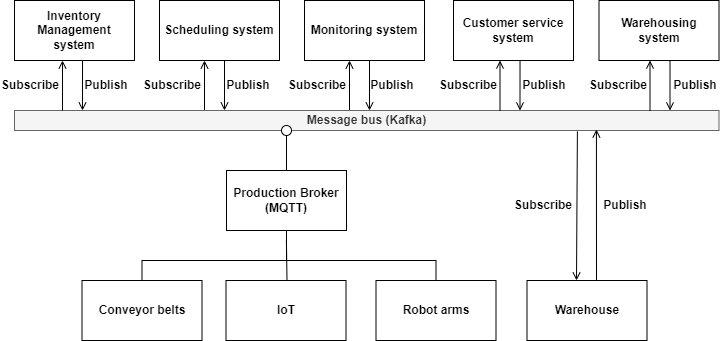
\includegraphics[width=250pt]{images/deployment-diagram.png}
    \caption{Initial deployment diagram of production system}
    \label{fig:deployment-diagram}
\end{figure}

By utilizing this setup, a message-oriented middleware as a layer between subsystems for abstracting and encapsulating functionality was needed as an interface to be used. Within the setup, Kafka as well as MQTT are being utilized as two different message buses, where MQTT is primarily intended for Internet of Things (IoT) devices on the production floor. Additionally, Kafka was to be utilized as the core broker solution to benefit scalability of a large production system.  


